%================================================
% PACKAGES AND THEMES
%================================================
\documentclass[t,aspectratio=169,xcolor=dvipsnames]{beamer}

\usetheme{SimplePlusAIC}

\usepackage{graphicx}
\usepackage{booktabs}
\usepackage{svg}
\usepackage{tcolorbox}
\usepackage{tikz}
\usetikzlibrary{shapes.geometric, arrows, positioning, fit, calc}
\usepackage{makecell}
\usepackage{listings}

\newcommand*{\defeq}{\stackrel{\text{def}}{=}}
\usepackage{setspace}
\usepackage[T1]{fontenc}
\usepackage{helvet}
\usepackage{amsmath}
\usepackage{ragged2e}
\usepackage{gensymb}

\usepackage[svgnames,table]{xcolor}
\arrayrulecolor{black}
\setlength{\arrayrulewidth}{0.20mm}
\renewcommand{\arraystretch}{1.35}

\newcommand{\tem}[1]{\textbf{\textcolor{red}{#1}}}

\lstset{
    basicstyle=\ttfamily\small,
    breaklines=true,
    columns=fullflexible,
    frame=none
}

%================================================
% TITLE PAGE
%================================================
\title[Locks \& Mutex]{Locks: Solusi untuk Critical Section}
\subtitle{Week 11: Lock Abstraction, Mutex, dan Atomic Instructions}
\author[informatika-itera.github.io/os]{informatika-itera.github.io/os}
\institute[ITERA]{Program Studi Teknik Informatika \\ Institut Teknologi Sumatera}
\date{\textcolor{nyublue}{2026}}

%================================================
% BEGIN DOCUMENT
%================================================
\begin{document}

\begin{frame}
    \titlepage
\end{frame}

\begin{frame}
    \frametitle{OUTLINE}
    \framesubtitle{Peta materi pertemuan ini}
    \small
    \begin{spacing}{1.15}
        \tableofcontents
    \end{spacing}
\end{frame}

\begin{frame}
    \frametitle{Capaian Pembelajaran}
    \framesubtitle{Tujuan setelah pertemuan selesai}
    \small
    \begin{enumerate}
        \item Menjelaskan apa itu lock dan mengapa kita membutuhkannya.
        \item Menggunakan \texttt{pthread\_mutex} untuk melindungi \textit{critical section}.
        \item Mengenali pola lock/unlock yang benar dan yang berbahaya.
        \item Menjelaskan bagaimana instruksi atomik (\texttt{test-and-set}, \texttt{compare-and-swap}) menjadi fondasi lock.
        \item Membandingkan spinlock dan mutex dari sisi kebenaran dan performa.
        \item Mengevaluasi lock menggunakan tiga syarat critical section dari minggu lalu.
    \end{enumerate}
    \begin{exampleblock}{Fokus Hari Ini}
        Kita mulai dari \tem{Bagian 1: Lock Abstraction} — intuisi, API, dan pola dasar.
    \end{exampleblock}
\end{frame}

%================================================
% BAGIAN 1: LOCK ABSTRACTION
%================================================
\section{Lock Abstraction}

\begin{frame}[plain]
    \begin{center}
        \vspace{3cm}
        \Huge\textbf{Lock Abstraction}
    \end{center}
\end{frame}

%--- Slide 1: Kembali ke masalah minggu lalu ---
\begin{frame}[fragile,shrink=3]
    \frametitle{Ingat Masalah Minggu Lalu?}
    \framesubtitle{Dua thread menghitung bersama — hasilnya malah salah}

    \begin{center}
    \begin{alertblock}{Kode yang terlihat benar, tapi hasilnya tidak bisa diprediksi}
\begin{lstlisting}[basicstyle=\ttfamily\scriptsize]
int counter = 0;   // dihitung bersama dua thread

void *increment(void *arg) {
    for (int i = 0; i < 1000000; i++)
        counter++;   // <-- di sinilah masalahnya
    return NULL;
}
\end{lstlisting}
    \end{alertblock}
    \end{center}

    \footnotesize
    Dua thread masing-masing menambah \texttt{counter} 1 juta kali.
    Harusnya \textbf{2.000.000} — tapi bisa lebih kecil.

    \begin{exampleblock}{Pertanyaan untuk kita hari ini}
        \centering
        Bagaimana agar \texttt{counter++} tidak bisa diganggu thread lain \tem{di tengah-tengah}?
    \end{exampleblock}
\end{frame}

%--- Slide 2: Ide dasar lock ---
\begin{frame}[shrink=5]
    \frametitle{Ide Dasarnya Sederhana: Kunci Pintu}
    \framesubtitle{Bayangkan ruangan yang hanya boleh diisi satu orang}

    \begin{columns}[T]
        \column{0.45\textwidth}
        \centering
        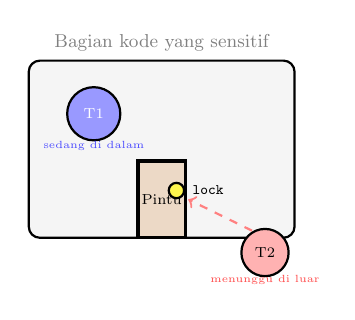
\begin{tikzpicture}[scale=0.75, transform shape]
            \draw[thick, rounded corners=4pt, fill=gray!8] (0,0.8) rectangle (4.5,3.8);
            \node[font=\small, gray] at (2.25, 4.1) {Bagian kode yang sensitif};

            \draw[very thick, fill=brown!30] (1.85, 0.8) rectangle (2.65, 2.1);
            \node[font=\scriptsize] at (2.25, 1.45) {Pintu};

            \draw[fill=yellow!70, thick] (2.5, 1.6) circle (0.13);
            \node[font=\scriptsize, right] at (2.65, 1.6) {\texttt{lock}};

            \draw[fill=blue!40, thick] (1.1, 2.9) circle (0.45);
            \node[font=\scriptsize, text=white] at (1.1, 2.9) {T1};
            \node[font=\tiny, blue!70] at (1.1, 2.35) {sedang di dalam};

            \draw[fill=red!30, thick] (4.0, 0.55) circle (0.40);
            \node[font=\scriptsize] at (4.0, 0.55) {T2};
            \node[font=\tiny, red!70] at (4.0, 0.08) {menunggu di luar};

            \draw[->, thick, red!50, dashed] (3.78, 0.92) -- (2.7, 1.45);
        \end{tikzpicture}

        \column{0.52\textwidth}
        \small
        Bayangkan ada \textbf{ruangan khusus} yang hanya boleh dimasuki \textbf{satu orang} pada satu waktu.

        \begin{itemize}
            \item Thread 1 masuk → \tem{kunci pintu dari dalam}
            \item Thread 2 datang → \textbf{tidak bisa masuk}, harus tunggu di luar
            \item Thread 1 selesai → \tem{buka kunci}
            \item Baru Thread 2 boleh masuk
        \end{itemize}

        \begin{exampleblock}{Inilah yang disebut \textbf{lock}}
            Lock = mekanisme yang memastikan hanya \tem{satu thread} yang boleh mengakses data penting pada satu waktu.
        \end{exampleblock}
    \end{columns}
\end{frame}

%--- Slide 3: Lock sebagai abstraksi ---
\begin{frame}
    \frametitle{Lock Punya Dua Perintah Saja}
    \framesubtitle{Cukup dua kata untuk mengatur giliran antar thread}
    \footnotesize

    \begin{columns}[T]
        \column{0.48\textwidth}
        \begin{block}{\textbf{acquire} — ``Saya mau masuk''}
            \begin{itemize}
                \item Thread minta izin masuk ke kode sensitif
                \item Belum ada yang di dalam → \textbf{langsung masuk}
                \item Sudah ada yang di dalam → \tem{tunggu dulu}
            \end{itemize}
        \end{block}

        \begin{block}{\textbf{release} — ``Saya sudah keluar''}
            \begin{itemize}
                \item Thread selesai, membuka kunci
                \item Thread lain yang menunggu \textbf{boleh masuk sekarang}
            \end{itemize}
        \end{block}

        \column{0.48\textwidth}
        \begin{exampleblock}{Aturan paling penting}
            \centering
            Pada satu waktu,\\
            \tem{hanya SATU thread}\\
            yang boleh memegang lock.
        \end{exampleblock}

        \begin{alertblock}{Urutan wajib}
            \centering
            \textbf{acquire}\\
            $\downarrow$\\
            kerjakan data sensitif\\
            $\downarrow$\\
            \textbf{release}
        \end{alertblock}
    \end{columns}
\end{frame}

%--- Slide 4: pthread_mutex API ---
\begin{frame}[fragile]
    \frametitle{Di C, Lock Disebut \texttt{mutex}}
    \framesubtitle{Empat langkah untuk memakai mutex — hafal urutannya}
    \footnotesize

    \begin{columns}[T]
        \column{0.54\textwidth}
\begin{lstlisting}[basicstyle=\ttfamily\scriptsize]
// 1: Siapkan variabel mutex
pthread_mutex_t lock;

// 2: Aktifkan sebelum dipakai
pthread_mutex_init(&lock, NULL);

// 3a: Kunci sebelum masuk
pthread_mutex_lock(&lock);
// ... kerjakan data sensitif ...

// 3b: Buka kunci setelah selesai
pthread_mutex_unlock(&lock);

// 4: Bersihkan di akhir program
pthread_mutex_destroy(&lock);
\end{lstlisting}

        \column{0.42\textwidth}
        \begin{block}{Empat langkah}
            \begin{enumerate}
                \item Buat variabel mutex
                \item \texttt{init} — hidupkan
                \item \texttt{lock} → kerja → \texttt{unlock}
                \item \texttt{destroy} — bersihkan
            \end{enumerate}
        \end{block}

        \begin{alertblock}{Aturan tidak boleh dilanggar}
            Setiap \texttt{lock} \tem{wajib} punya pasangan \texttt{unlock}.
        \end{alertblock}
    \end{columns}
\end{frame}

%--- Slide 5: Fix counter++ ---
\begin{frame}[fragile,shrink=8]
    \frametitle{Sekarang Kita Perbaiki \texttt{counter++}}
    \framesubtitle{Tambahkan lock dan unlock di sekitar baris yang bermasalah}
    \footnotesize

    \begin{columns}[T]
        \column{0.50\textwidth}
        \begin{alertblock}{Versi lama — bermasalah}
\begin{lstlisting}[basicstyle=\ttfamily\scriptsize]
int counter = 0;

void *increment(void *arg) {
    for (int i = 0; i < 1000000; i++)
        counter++;   // thread lain bisa
                     // menyela di sini!
    return NULL;
}
\end{lstlisting}
        \end{alertblock}

        \column{0.46\textwidth}
        \begin{exampleblock}{Versi baru — aman}
\begin{lstlisting}[basicstyle=\ttfamily\scriptsize]
int counter = 0;
pthread_mutex_t lock;   // tambahan

void *increment(void *arg) {
    for (int i = 0; i < 1000000; i++) {
        pthread_mutex_lock(&lock);
        counter++;   // aman sekarang
        pthread_mutex_unlock(&lock);
    }
    return NULL;
}
\end{lstlisting}
        \end{exampleblock}
    \end{columns}

    \begin{block}{Kenapa sekarang aman?}
        Saat T1 di antara \texttt{lock} dan \texttt{unlock}, T2 \tem{tidak bisa masuk}.
        LOAD–ADD–STORE tidak bisa disela. Hasil selalu tepat \textbf{2.000.000}.
    \end{block}
\end{frame}

%--- Slide 6: Visualisasi timeline mutex ---
\begin{frame}
    \frametitle{Lihat Apa yang Terjadi di Garis Waktu}
    \framesubtitle{Thread 2 sabar menunggu sampai Thread 1 benar-benar selesai}

    \centering
    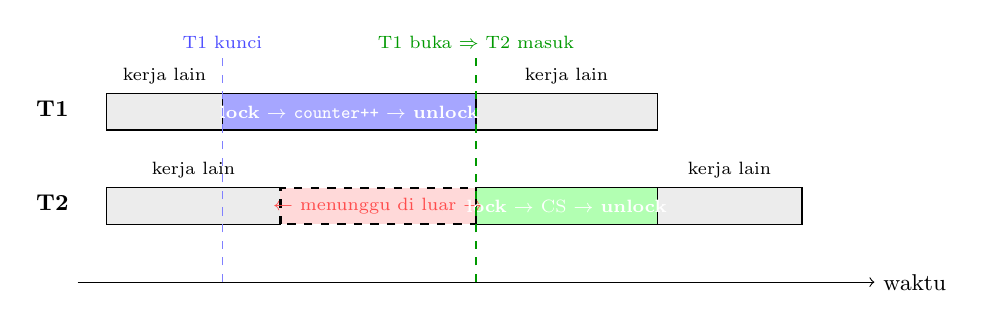
\begin{tikzpicture}[scale=0.92, transform shape]
        \draw[->] (0,0) -- (11,0) node[right, font=\small]{waktu};

        % Thread 1
        \node[left, font=\small] at (0, 2.4) {\textbf{T1}};
        \draw[fill=gray!15] (0.4, 2.1) rectangle (2.0, 2.6);
        \draw[fill=blue!35] (2.0, 2.1) rectangle (5.5, 2.6);
        \draw[fill=gray!15] (5.5, 2.1) rectangle (8.0, 2.6);

        \node[font=\scriptsize] at (1.2,  2.85) {kerja lain};
        \node[font=\scriptsize, white] at (3.75, 2.35) {\textbf{lock} $\to$ \texttt{counter++} $\to$ \textbf{unlock}};
        \node[font=\scriptsize] at (6.75, 2.85) {kerja lain};

        % Thread 2
        \node[left, font=\small] at (0, 1.1) {\textbf{T2}};
        \draw[fill=gray!15] (0.4, 0.8) rectangle (2.8, 1.3);
        \draw[fill=red!15,  dashed, thick] (2.8, 0.8) rectangle (5.5, 1.3);
        \draw[fill=green!30] (5.5, 0.8) rectangle (8.0, 1.3);
        \draw[fill=gray!15] (8.0, 0.8) rectangle (10.0, 1.3);

        \node[font=\scriptsize] at (1.6,  1.55) {kerja lain};
        \node[font=\scriptsize, red!70] at (4.15, 1.05) {$\leftarrow$ menunggu di luar $\rightarrow$};
        \node[font=\scriptsize, white] at (6.75, 1.05) {\textbf{lock} $\to$ CS $\to$ \textbf{unlock}};
        \node[font=\scriptsize] at (9.0,  1.55) {kerja lain};

        \draw[dashed, blue!50] (2.0, 0) -- (2.0, 3.1);
        \node[font=\scriptsize, blue!70, above] at (2.0, 3.1) {T1 kunci};

        \draw[dashed, green!60!black] (5.5, 0) -- (5.5, 3.1);
        \node[font=\scriptsize, green!60!black, above] at (5.5, 3.1) {T1 buka $\Rightarrow$ T2 masuk};
    \end{tikzpicture}

    \vspace{0.2cm}
    \small
    Perhatikan: bagian biru T1 dan bagian hijau T2 \tem{tidak pernah terjadi di waktu yang sama}.\\
    Itulah yang kita inginkan — tidak ada yang saling menyela.
\end{frame}

%--- Slide 7: Pola lock/unlock yang benar ---
\begin{frame}[fragile]
    \frametitle{Hati-Hati: Jangan Lupa Membuka Kunci}
    \framesubtitle{Kesalahan kecil ini bisa membuat program berhenti selamanya}
    \small

    \begin{columns}[T]
        \column{0.48\textwidth}
        \begin{exampleblock}{\checkmark\ Pola yang benar}
\begin{lstlisting}[basicstyle=\ttfamily\scriptsize]
pthread_mutex_lock(&lock);
counter++;   // kerja
pthread_mutex_unlock(&lock);
// kunci sudah dibuka, aman
\end{lstlisting}
            Setiap \texttt{lock} punya pasangan \texttt{unlock}.\\
            Thread lain tidak akan kehabisan giliran.
        \end{exampleblock}

        \column{0.48\textwidth}
        \begin{alertblock}{\texttimes\ Pola berbahaya}
\begin{lstlisting}[basicstyle=\ttfamily\scriptsize]
pthread_mutex_lock(&lock);
if (ada_error) return;
// BAHAYA: unlock terlewat!
counter++;
pthread_mutex_unlock(&lock);
\end{lstlisting}
            Kalau \texttt{return} dijalankan, \texttt{unlock} terlewat.\\
            Thread lain \tem{menunggu selamanya}.
        \end{alertblock}
    \end{columns}

    \begin{block}{Cara mengingat}
        Bayangkan kamu mengunci pintu kamar mandi lalu keluar lewat jendela.
        Pintu tetap terkunci — orang berikutnya tidak bisa masuk!
    \end{block}
\end{frame}

%--- Slide 8: Apa yang terjadi saat lock diambil ---
\begin{frame}
    \frametitle{Saat Menunggu, Thread Melakukan Apa?}
    \framesubtitle{Ada dua cara menunggu — dan keduanya punya konsekuensi berbeda}
    \footnotesize

    \begin{columns}[T]
        \column{0.48\textwidth}
        \begin{block}{Cara 1: Tidur dulu (Mutex)}
            \begin{enumerate}
                \item Thread minta lock
                \item Lock belum bebas → OS \textbf{tidurkan thread}
                \item Thread berhenti, tidak pakai CPU
                \item Lock dilepas → OS \textbf{bangunkan thread}
            \end{enumerate}
            \textit{Ambil nomor antrean, duduk sampai dipanggil.}
        \end{block}

        \column{0.48\textwidth}
        \begin{alertblock}{Cara 2: Terus Cek (Spinlock)}
            \begin{enumerate}
                \item Thread minta lock
                \item Lock belum bebas → thread \tem{loop terus}
                \item \texttt{while (terkunci) \{ cek lagi \}}
                \item Lock dilepas → keluar dari loop
            \end{enumerate}
            \textit{Berdiri di kasir dan terus tanya ``sudah bisa belum?''}
        \end{alertblock}
    \end{columns}

    \begin{exampleblock}{Mana yang lebih baik?}
        Mutex hemat CPU (thread tidur). Spinlock lebih cepat jika tunggu \textbf{sangat singkat}, tapi boros CPU kalau lama.
    \end{exampleblock}
\end{frame}

%--- Slide 9: Hands-on ---
\begin{frame}[fragile,shrink=5]
    \frametitle{Sekarang Kita Coba Sendiri}
    \framesubtitle{Jalankan dua program, lihat perbedaannya dengan mata kepala sendiri}
    \small

    \begin{columns}[T]
        \column{0.50\textwidth}
        \begin{alertblock}{Program 1: Tanpa mutex}
\begin{lstlisting}[basicstyle=\ttfamily\scriptsize]
cd 4_handson_code/week11
gcc -Wall -pthread -O0 \
    -o race 01_race.c
./race
\end{lstlisting}
            Jalankan \textbf{3 kali}. Catat hasilnya.\\
            Apakah selalu sama?
        \end{alertblock}

        \column{0.46\textwidth}
        \begin{exampleblock}{Program 2: Dengan mutex}
\begin{lstlisting}[basicstyle=\ttfamily\scriptsize]
gcc -Wall -pthread -O0 \
    -o mutex 02_mutex.c
./mutex
\end{lstlisting}
            Jalankan \textbf{3 kali}. Catat hasilnya.\\
            Apakah selalu sama?
        \end{exampleblock}
    \end{columns}

    \begin{block}{Catat tiga hal ini}
        \footnotesize
        \begin{enumerate}
            \item \texttt{race}: apakah hasilnya berubah-ubah? Berapa jauh dari 2.000.000?
            \item \texttt{mutex}: apakah hasilnya selalu 2.000.000?
            \item Mana yang lebih cepat, dan mengapa?
        \end{enumerate}
    \end{block}
\end{frame}

%--- Slide 10: Checkpoint ---
\begin{frame}
    \frametitle{Checkpoint: Paham Sampai Mana?}
    \framesubtitle{Empat pertanyaan — jawab tanpa melihat slide sebelumnya}
    \small

    \begin{enumerate}
        \item Lock punya dua perintah utama. Sebutkan keduanya dan jelaskan apa yang terjadi kalau lock sedang dipakai thread lain.
        \item Sebutkan empat fungsi \texttt{pthread\_mutex} secara berurutan — dari deklarasi hingga selesai dipakai.
        \item Kenapa kode seperti ini berbahaya?
        \texttt{lock() → if error return → ... → unlock()}
        \item Apa bedanya mutex dan spinlock dari sisi \textbf{apa yang dilakukan thread} saat menunggu?
    \end{enumerate}

    \begin{block}{Jawaban}
        \footnotesize
        \begin{enumerate}
            \item \texttt{acquire} (kunci) dan \texttt{release} (buka). Kalau sudah dipakai, thread lain harus tunggu.
            \item \texttt{init} → \texttt{lock} → \textit{kerja} → \texttt{unlock} → \texttt{destroy}.
            \item Jalur \texttt{return} melewati \texttt{unlock} — kunci tidak pernah dibuka, thread lain menunggu selamanya.
            \item Mutex: thread tidur, tidak pakai CPU. Spinlock: thread terus cek dalam loop, CPU tetap terpakai.
        \end{enumerate}
    \end{block}
\end{frame}

%================================================
% BAGIAN 2: HARDWARE FOUNDATION
%================================================
\section{Hardware Foundation: Instruksi Atomik}

\begin{frame}[plain]
    \begin{center}
        \vspace{3cm}
        \Huge\textbf{Hardware Foundation}\\[0.4em]
        \Large\textit{Mengapa Software Saja Tidak Cukup?}
    \end{center}
\end{frame}

%--- Slide 11: Kenapa software-only gagal ---
\begin{frame}[fragile,shrink=5]
    \frametitle{Percobaan Dulu: Buat Lock Sendiri dari Kode}
    \framesubtitle{Minggu lalu kita coba — hasilnya masih bisa salah. Kenapa?}
    \footnotesize

    \begin{columns}[T]
        \column{0.50\textwidth}
        \begin{alertblock}{Ide awal: pakai variabel ``bendera''}
\begin{lstlisting}[basicstyle=\ttfamily\scriptsize]
int flag = 0;   // 0 = bebas, 1 = terkunci

void lock() {
    while (flag == 1) { }  // tunggu
    flag = 1;              // ambil kunci
}

void unlock() {
    flag = 0;
}
\end{lstlisting}
        \end{alertblock}

        \column{0.46\textwidth}
        \begin{block}{Kelihatannya masuk akal}
            \begin{itemize}
                \item Cek dulu: apakah flag bebas?
                \item Kalau bebas → set flag = 1 (kunci)
                \item Kalau sudah dikunci → tunggu
            \end{itemize}
        \end{block}

        \begin{exampleblock}{Pertanyaan}
            \centering
            Ada yang salah di sini.\\
            Bisakah kamu menemukan lubangnya?
        \end{exampleblock}
    \end{columns}
\end{frame}

%--- Slide 12: Masalahnya ada di mana ---
\begin{frame}
    \frametitle{Masalahnya: Ada Jeda Berbahaya di Antara Dua Langkah}
    \framesubtitle{CHECK dan SET adalah dua instruksi terpisah — dan bisa disela!}

    \centering
    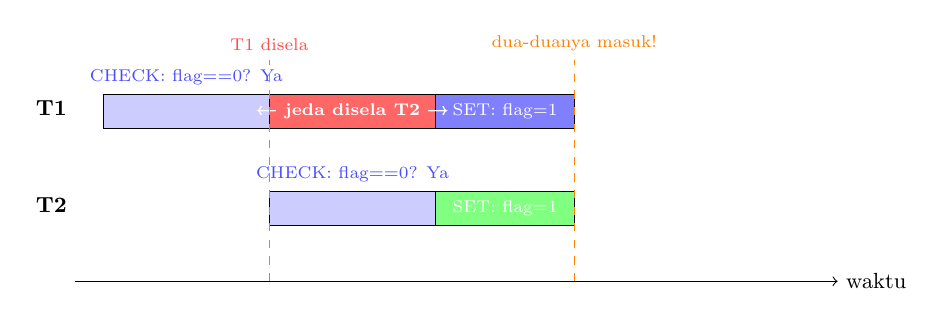
\begin{tikzpicture}[scale=0.88, transform shape]
        \draw[->] (0,0) -- (11,0) node[right, font=\small]{waktu};

        % T1
        \node[left, font=\small] at (0,2.5) {\textbf{T1}};
        \draw[fill=blue!20]  (0.4,2.2) rectangle (2.8,2.7);
        \draw[fill=red!60]   (2.8,2.2) rectangle (5.2,2.7);
        \draw[fill=blue!50]  (5.2,2.2) rectangle (7.2,2.7);

        \node[font=\scriptsize, blue!70] at (1.6, 2.95)  {CHECK: flag==0? Ya};
        \node[font=\scriptsize, white]   at (4.0, 2.45)  {\textbf{← jeda disela T2 →}};
        \node[font=\scriptsize, white]   at (6.2, 2.45)  {SET: flag=1};

        % T2
        \node[left, font=\small] at (0,1.1) {\textbf{T2}};
        \draw[fill=blue!20]  (2.8,0.8) rectangle (5.2,1.3);
        \draw[fill=green!50] (5.2,0.8) rectangle (7.2,1.3);

        \node[font=\scriptsize, blue!70] at (4.0, 1.55) {CHECK: flag==0? Ya};
        \node[font=\scriptsize, white]   at (6.2, 1.05) {SET: flag=1};

        % markers
        \draw[dashed, red!60] (2.8,0) -- (2.8,3.2);
        \node[font=\scriptsize, red!70, above] at (2.8,3.2) {T1 disela};

        \draw[dashed, orange] (7.2,0) -- (7.2,3.2);
        \node[font=\scriptsize, orange, above] at (7.2,3.2) {dua-duanya masuk!};
    \end{tikzpicture}

    \vspace{0.2cm}
    \small
    T1 sudah cek flag = 0, tapi belum sempat set flag = 1.\\
    T2 masuk di celah itu — cek juga 0 — keduanya \tem{lolos bersama}. Kunci gagal.
\end{frame}

%--- Slide 13: Solusi — butuh satu langkah atomik ---
\begin{frame}[shrink=5]
    \frametitle{Solusinya: Satu Langkah yang Tidak Bisa Disela}
    \framesubtitle{Kita butuh CHECK dan SET terjadi sekaligus — tidak ada jeda}
    \small

    \begin{columns}[T]
        \column{0.48\textwidth}
        \begin{alertblock}{Masalah software-only}
            \begin{enumerate}
                \item CHECK (cek flag)
                \item \textit{--- bisa disela di sini ---}
                \item SET (ubah flag)
            \end{enumerate}
            Dua langkah terpisah = ada peluang masalah.
        \end{alertblock}

        \column{0.48\textwidth}
        \begin{exampleblock}{Yang kita butuhkan}
            \begin{enumerate}
                \item CHECK + SET \tem{sekaligus}
                \item Tidak ada yang bisa masuk di tengah
                \item Dilakukan dalam \textbf{satu instruksi CPU}
            \end{enumerate}
            Satu langkah = tidak ada celah.
        \end{exampleblock}
    \end{columns}

    \vspace{0.4em}
    \begin{block}{Inilah yang dimaksud \tem{Atomik}}
        \centering
        Kata \textit{atom} berarti ``tidak bisa dibagi''.\\
        Instruksi atomik = instruksi yang dijalankan \textbf{utuh atau tidak sama sekali}.\\
        CPU menjamin tidak ada thread lain yang bisa menyela di tengahnya.
    \end{block}
\end{frame}

%--- Slide 14: Test-and-Set ---
\begin{frame}[fragile,shrink=10]
    \frametitle{Test-and-Set: Instruksi Atomik Pertama}
    \framesubtitle{Satu instruksi, dua hal sekaligus — baca nilai lama, lalu langsung ganti}
    \small

    \begin{columns}[T]
        \column{0.50\textwidth}
        \begin{block}{Cara kerja (pseudocode)}
\begin{lstlisting}[basicstyle=\ttfamily\scriptsize]
// Ini SATU instruksi CPU
// tidak bisa disela
int TestAndSet(int *flag, int new) {
    int old = *flag;  // baca nilai lama
    *flag = new;      // langsung tulis baru
    return old;       // kembalikan nilai lama
}
\end{lstlisting}
        \end{block}

        \begin{block}{Pakai untuk lock}
\begin{lstlisting}[basicstyle=\ttfamily\scriptsize]
// lock berhasil jika nilai lama = 0
// lock gagal jika nilai lama = 1
while (TestAndSet(&flag, 1) == 1)
    ; // masih terkunci, tunggu
// sekarang kita yang pegang lock
\end{lstlisting}
        \end{block}

        \column{0.46\textwidth}
        \begin{exampleblock}{Analogi kasir}
            Bayangkan mesin tiket yang hanya punya satu tombol:\\[0.3em]
            \textit{``Ambil nomor antrean saat ini \textbf{dan} langsung ganti ke nomor berikutnya.''} \\[0.3em]
            Dua hal itu terjadi bersamaan — tidak ada yang bisa menyerobot di antaranya.
        \end{exampleblock}

        \begin{alertblock}{Kuncinya}
            Nilai lama dikembalikan \tem{sebelum} nilai baru ditulis.\\
            Jika dapat 0 → kita berhasil kunci.\\
            Jika dapat 1 → orang lain duluan.
        \end{alertblock}
    \end{columns}
\end{frame}

%--- Slide 15: Spinlock dengan Test-and-Set ---
\begin{frame}[fragile,shrink=10]
    \frametitle{Bangun Spinlock dengan Test-and-Set}
    \framesubtitle{Ini adalah spinlock paling sederhana yang bisa dibuat di C}
    \footnotesize

    \begin{columns}[T]
        \column{0.54\textwidth}
\begin{lstlisting}[basicstyle=\ttfamily\scriptsize]
#include <pthread.h>

int flag = 0;   // 0=bebas, 1=terkunci

void spin_lock(int *f) {
    // __sync_lock_test_and_set adalah
    // versi C dari instruksi Test-and-Set
    while (__sync_lock_test_and_set(f, 1) == 1)
        ;   // putar terus sampai dapat 0
}

void spin_unlock(int *f) {
    // tulis 0 dengan cara atomik
    __sync_lock_release(f);
}

// Pemakaian:
spin_lock(&flag);
counter++;   // aman sekarang
spin_unlock(&flag);
\end{lstlisting}

        \column{0.42\textwidth}
        \begin{block}{Cara baca kodenya}
            \begin{itemize}
                \item \texttt{\_\_sync\_lock\_test\_and\_set} = Test-and-Set bawaan GCC
                \item Kalau dapat 1 → orang lain masih di dalam, terus putar
                \item Kalau dapat 0 → kita berhasil masuk, tulis 1 sekaligus
            \end{itemize}
        \end{block}

        \begin{alertblock}{Ingat}
            Spinlock \tem{sibukkan CPU} selama menunggu.\\
            Cocok hanya untuk tunggu sangat singkat.
        \end{alertblock}
    \end{columns}
\end{frame}

%--- Slide 16: Compare-and-Swap ---
\begin{frame}[fragile,shrink=10]
    \frametitle{Compare-and-Swap: Instruksi Atomik yang Lebih Pintar}
    \framesubtitle{Tukar nilai hanya jika kondisinya terpenuhi — kalau tidak, biarkan}
    \small

    \begin{columns}[T]
        \column{0.50\textwidth}
        \begin{block}{Cara kerja (pseudocode)}
\begin{lstlisting}[basicstyle=\ttfamily\scriptsize]
// Ini SATU instruksi CPU
int CompareAndSwap(int *addr,
                  int expected,
                  int new) {
    if (*addr == expected) {
        *addr = new;   // tukar!
        return 1;      // berhasil
    }
    return 0;          // tidak ditukar
}
\end{lstlisting}
        \end{block}

        \column{0.46\textwidth}
        \begin{block}{Bedanya dengan Test-and-Set}
            \begin{tabular}{p{0.44\textwidth} p{0.44\textwidth}}
                \textbf{Test-and-Set} & \textbf{Compare-and-Swap} \\
                \hline
                Selalu tukar & Tukar \textit{hanya jika} nilai cocok \\
                Kembalikan nilai lama & Kembalikan sukses/gagal \\
                Sederhana & Lebih fleksibel \\
            \end{tabular}
        \end{block}

        \begin{exampleblock}{Analogi}
            Seperti memasukkan koin ke loker:\\
            \textit{``Buka hanya jika kunci cocok — jika tidak, tidak berubah apa-apa.''}
        \end{exampleblock}
    \end{columns}

\end{frame}

%--- Slide 17: Visualisasi atomik vs non-atomik ---
\begin{frame}
    \frametitle{Lihat Bedanya: Atomik vs Non-Atomik}
    \framesubtitle{Instruksi atomik menutup ``jendela bahaya'' yang ada di software-only}

    \centering
    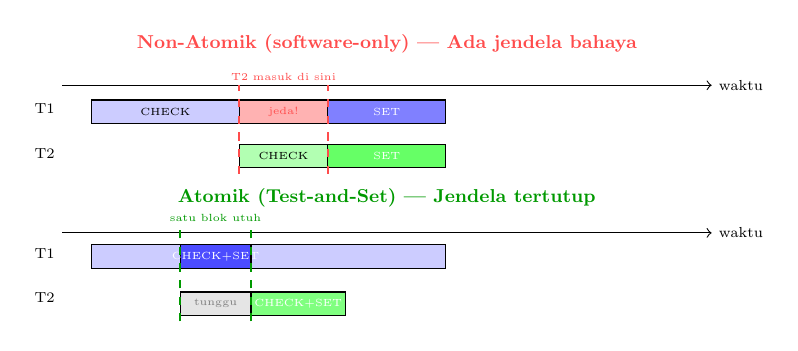
\begin{tikzpicture}[scale=0.75, transform shape]

        % --- Non-atomik (atas) ---
        \node[font=\small\bfseries, red!70] at (5.5, 5.2) {Non-Atomik (software-only) — Ada jendela bahaya};
        \draw[->] (0,4.5) -- (11,4.5) node[right, font=\scriptsize]{waktu};

        \node[left, font=\scriptsize] at (0,4.1) {T1};
        \draw[fill=blue!20]  (0.5,3.85) rectangle (3.0,4.25);
        \draw[fill=red!30]   (3.0,3.85) rectangle (4.5,4.25);
        \draw[fill=blue!50]  (4.5,3.85) rectangle (6.5,4.25);
        \node[font=\tiny] at (1.75,4.05) {CHECK};
        \node[font=\tiny, red!70] at (3.75,4.05) {jeda!};
        \node[font=\tiny, white] at (5.5,4.05) {SET};

        \node[left, font=\scriptsize] at (0,3.35) {T2};
        \draw[fill=green!30] (3.0,3.1) rectangle (4.5,3.5);
        \draw[fill=green!60] (4.5,3.1) rectangle (6.5,3.5);
        \node[font=\tiny] at (3.75,3.3) {CHECK};
        \node[font=\tiny, white] at (5.5,3.3) {SET};

        \draw[dashed, red!70, thick] (3.0,3.0) -- (3.0,4.5);
        \draw[dashed, red!70, thick] (4.5,3.0) -- (4.5,4.5);
        \node[font=\tiny, red!70] at (3.75,4.65) {T2 masuk di sini};

        % --- Atomik (bawah) ---
        \node[font=\small\bfseries, green!60!black] at (5.5, 2.6) {Atomik (Test-and-Set) — Jendela tertutup};
        \draw[->] (0,2.0) -- (11,2.0) node[right, font=\scriptsize]{waktu};

        \node[left, font=\scriptsize] at (0,1.65) {T1};
        \draw[fill=blue!20]  (0.5,1.4) rectangle (2.0,1.8);
        \draw[fill=blue!70]  (2.0,1.4) rectangle (3.2,1.8);
        \draw[fill=blue!20]  (3.2,1.4) rectangle (6.5,1.8);
        \node[font=\tiny, white] at (2.6,1.6) {CHECK+SET};

        \node[left, font=\scriptsize] at (0,0.9) {T2};
        \draw[fill=gray!20]  (2.0,0.6) rectangle (3.2,1.0);
        \draw[fill=green!50] (3.2,0.6) rectangle (4.8,1.0);
        \node[font=\tiny, gray] at (2.6,0.8) {tunggu};
        \node[font=\tiny, white] at (4.0,0.8) {CHECK+SET};

        \draw[dashed, green!60!black, thick] (2.0,0.5) -- (2.0,2.1);
        \draw[dashed, green!60!black, thick] (3.2,0.5) -- (3.2,2.1);
        \node[font=\tiny, green!60!black] at (2.6,2.25) {satu blok utuh};
    \end{tikzpicture}

\end{frame}

%--- Slide 18: Hands-on spinlock ---
\begin{frame}[fragile,shrink=5]
    \frametitle{Coba Sendiri: Spinlock vs Mutex}
    \framesubtitle{Dua cara lock — satu sibuk menunggu, satu tidur menunggu}
    \small

    \begin{columns}[T]
        \column{0.50\textwidth}
        \begin{alertblock}{Program 3: Spinlock}
\begin{lstlisting}[basicstyle=\ttfamily\scriptsize]
gcc -Wall -pthread -O0 \
    -o spin 03_spinlock.c
./spin
\end{lstlisting}
            Jalankan \textbf{3 kali}. Catat hasilnya.\\
            Apakah selalu 2.000.000?
        \end{alertblock}

        \begin{block}{Bandingkan dua lock}
\begin{lstlisting}[basicstyle=\ttfamily\scriptsize]
time ./mutex   # mutex
time ./spin    # spinlock
\end{lstlisting}
            Mana yang lebih cepat?
        \end{block}

        \column{0.46\textwidth}
        \begin{exampleblock}{Yang perlu diobservasi}
            \begin{enumerate}
                \item Keduanya harus menghasilkan 2.000.000 — kebenaran sama
                \item Kecepatan bisa berbeda — lihat output \texttt{time}
                \item Coba pantau CPU: \texttt{top} saat spinlock berjalan
            \end{enumerate}
        \end{exampleblock}

        \begin{block}{Diskusi}
            \footnotesize
            Spinlock mungkin lebih cepat karena tidak ada overhead sleep/wake. Tapi CPU-nya 100\%. Mutex lebih hemat — tapi ada biaya bangun-tidur. Mana yang cocok untuk situasi apa?
        \end{block}
    \end{columns}
\end{frame}

%--- Slide 19: Checkpoint 2 ---
\begin{frame}[shrink=15]
    \frametitle{Checkpoint 2: Hardware Foundation}
    \framesubtitle{Empat pertanyaan — jawab tanpa melihat slide sebelumnya}
    \small

    \begin{enumerate}
        \item Kenapa flag biasa (variabel \texttt{int}) tidak cukup untuk membuat lock yang benar meskipun logikanya kelihatan masuk akal?
        \item Apa yang dimaksud instruksi \textbf{atomik}? Berikan satu contoh hal yang dijamin oleh instruksi atomik.
        \item Jelaskan cara kerja Test-and-Set dalam satu atau dua kalimat. Nilai apa yang dikembalikan jika kunci \textbf{sudah diambil} orang lain?
        \item Apa perbedaan utama antara Test-and-Set dan Compare-and-Swap?
    \end{enumerate}

    \begin{block}{Jawaban}
        \footnotesize
        \begin{enumerate}
            \item CHECK dan SET adalah dua instruksi terpisah — ada jeda di antaranya. Thread lain bisa masuk di celah itu.
            \item Instruksi yang dijalankan utuh, tidak bisa disela di tengah. Contoh: Test-and-Set menjamin baca dan tulis terjadi sekaligus.
            \item Test-and-Set membaca nilai lama lalu langsung menulis nilai baru dalam satu instruksi. Jika kunci sudah diambil (flag=1), ia kembalikan 1.
            \item Test-and-Set selalu menulis nilai baru. Compare-and-Swap hanya menulis jika nilai saat ini sama dengan yang diharapkan — lebih selektif.
        \end{enumerate}
    \end{block}
\end{frame}

%================================================
% BAGIAN 3: LOCK CORRECTNESS & FAIRNESS
%================================================
\section{Kebenaran dan Keadilan Lock}

\begin{frame}[plain]
    \begin{center}
        \vspace{3cm}
        \Huge\textbf{Kebenaran dan Keadilan Lock}\\[0.4em]
        \Large\textit{Apakah Lock Kita Sudah Benar-Benar Aman?}
    \end{center}
\end{frame}

%--- Slide 20: Tiga syarat critical section ---
\begin{frame}[shrink=5]
    \frametitle{Ingat Tiga Syarat dari Minggu Lalu?}
    \framesubtitle{Lock harus memenuhi ketiganya — mari kita periksa satu per satu}
    \footnotesize

    \begin{columns}[T]
        \column{0.48\textwidth}
        \begin{block}{Tiga syarat critical section}
            \begin{enumerate}
                \item \textbf{Mutual Exclusion}\\
                      Hanya satu thread di dalam pada satu waktu.
                \vspace{0.3em}
                \item \textbf{Progress}\\
                      Kalau tidak ada yang di dalam, thread yang mau masuk tidak boleh diblokir selamanya.
                \vspace{0.3em}
                \item \textbf{Bounded Waiting}\\
                      Setiap thread yang menunggu pasti mendapat giliran — tidak boleh menunggu selamanya.
            \end{enumerate}
        \end{block}

        \column{0.48\textwidth}
        \begin{exampleblock}{Pertanyaan yang kita jawab hari ini}
            \centering
            Apakah \texttt{pthread\_mutex}\\
            dan \textbf{spinlock} memenuhi\\
            ketiga syarat ini?
        \end{exampleblock}

        \begin{alertblock}{Spoiler}
            Syarat 1 terpenuhi. Syarat 3 \tem{belum tentu} — tergantung implementasi.
        \end{alertblock}
    \end{columns}
\end{frame}

%--- Slide 21: Mutual exclusion terpenuhi ---
\begin{frame}[shrink=18]
    \frametitle{Syarat 1: Mutual Exclusion — Terpenuhi}
    \framesubtitle{Ini adalah tujuan utama lock — dan keduanya berhasil}
    \footnotesize

    \begin{columns}[T]
        \column{0.48\textwidth}
        \begin{exampleblock}{\checkmark\ Mutex}
            \begin{itemize}
                \item Thread minta lock → OS periksa
                \item Kalau sudah ada yang di dalam → thread \textbf{tidur}, tidak bisa masuk
                \item Hanya satu thread aktif di critical section
            \end{itemize}
        \end{exampleblock}

        \begin{exampleblock}{\checkmark\ Spinlock}
            \begin{itemize}
                \item Thread minta lock → Test-and-Set atomik
                \item Kalau sudah diambil → thread \textbf{loop}, tidak bisa masuk
                \item Hanya satu thread berhasil ambil lock (nilai lama = 0)
            \end{itemize}
        \end{exampleblock}

        \column{0.48\textwidth}
        \begin{block}{Kenapa keduanya lulus?}
            Karena instruksi di bawahnya \tem{atomik}.\\[0.5em]
            Mutex pakai syscall OS yang atomic.\\
            Spinlock pakai Test-and-Set atomic.\\[0.5em]
            Tidak ada ``celah'' untuk dua thread masuk bersamaan.
        \end{block}
    \end{columns}

    \vspace{0.3em}
    \begin{block}{}
        \centering
        \footnotesize
        Mutual exclusion = tujuan utama lock. Kedua jenis lock \textbf{lulus syarat ini}.
    \end{block}
\end{frame}

%--- Slide 22: Fairness dan starvation ---
\begin{frame}[shrink=8]
    \frametitle{Syarat 3: Bounded Waiting — Belum Tentu Terpenuhi}
    \framesubtitle{Apakah setiap thread yang menunggu pasti dapat giliran?}
    \footnotesize

    \begin{columns}[T]
        \column{0.48\textwidth}
        \begin{exampleblock}{\checkmark\ Mutex (biasanya)}
            OS menyimpan \textbf{antrian} thread yang menunggu.\\
            Saat lock dilepas, OS pilih thread berikutnya dari antrian.\\[0.3em]
            Seperti antrean kasir — siapa datang duluan, dilayani duluan.\\[0.3em]
            \textit{Tapi bergantung pada implementasi OS.}
        \end{exampleblock}

        \column{0.48\textwidth}
        \begin{alertblock}{\texttimes\ Spinlock — tidak ada jaminan}
            Spinlock \tem{tidak punya antrian}.\\
            Saat flag = 0, semua thread yang spinning berlomba pakai Test-and-Set.\\[0.3em]
            Thread mana yang menang? \textbf{Tidak ada yang tahu.}\\[0.3em]
            Thread tertentu bisa kalah terus — \tem{starvation}.
        \end{alertblock}
    \end{columns}

    \begin{block}{Apa itu Starvation?}
        \centering
        Thread \textit{kelaparan} = thread menunggu sangat lama (atau selamanya) karena thread lain terus-terusan mendapat giliran duluan.
    \end{block}
\end{frame}

%--- Slide 23: Checkpoint 3 ---
\begin{frame}[shrink=20]
    \frametitle{Checkpoint 3: Kebenaran Lock}
    \framesubtitle{Tiga pertanyaan — jawab tanpa melihat slide sebelumnya}
    \small

    \begin{enumerate}
        \item Sebutkan tiga syarat yang harus dipenuhi oleh sebuah mekanisme critical section.
        \item Mengapa mutex dan spinlock keduanya memenuhi syarat \textbf{Mutual Exclusion}? Apa yang menjamin hal itu?
        \item Apa yang dimaksud \textit{starvation}? Mengapa spinlock lebih rentan terhadap starvation dibandingkan mutex?
    \end{enumerate}

    \begin{block}{Jawaban}
        \footnotesize
        \begin{enumerate}
            \item Mutual Exclusion, Progress, Bounded Waiting.
            \item Keduanya menggunakan instruksi atomik di bawahnya (syscall OS untuk mutex, Test-and-Set untuk spinlock) sehingga tidak ada celah untuk dua thread masuk bersamaan.
            \item Starvation = thread menunggu sangat lama karena selalu kalah bersaing. Spinlock tidak punya antrian — saat lock bebas, semua thread spinning berlomba tanpa urutan, sehingga thread tertentu bisa selalu kalah.
        \end{enumerate}
    \end{block}
\end{frame}

%================================================
% BAGIAN 4: DEADLOCK
%================================================
\section{Deadlock}

\begin{frame}[plain]
    \begin{center}
        \vspace{3cm}
        \Huge\textbf{Deadlock}\\[0.4em]
        \Large\textit{Ketika Tidak Ada yang Bisa Maju}
    \end{center}
\end{frame}

%--- Slide 24: Apa itu deadlock ---
\begin{frame}[shrink=5]
    \frametitle{Deadlock: Dua Thread Saling Tunggu}
    \framesubtitle{Ini lebih berbahaya dari lupa unlock — tidak ada yang bisa maju}
    \footnotesize

    \begin{columns}[T]
        \column{0.50\textwidth}
        \begin{alertblock}{Skenario}
            \begin{tabular}{p{0.44\textwidth} p{0.44\textwidth}}
                \textbf{Thread 1} & \textbf{Thread 2} \\
                \hline
                \texttt{lock(A)} & \texttt{lock(B)} \\
                \textit{(pegang A)} & \textit{(pegang B)} \\
                \texttt{lock(B)...} & \texttt{lock(A)...} \\
                \textit{tunggu B} & \textit{tunggu A} \\
            \end{tabular}
        \end{alertblock}

        \begin{block}{Hasilnya}
            T1 tunggu B yang dipegang T2.\\
            T2 tunggu A yang dipegang T1.\\
            \tem{Keduanya menunggu selamanya.}
        \end{block}

        \column{0.46\textwidth}

        \centering
        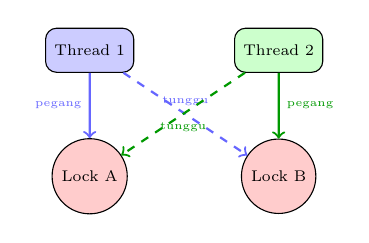
\begin{tikzpicture}[scale=0.8, transform shape]
            \node[draw, fill=blue!20, rounded corners, minimum width=1.4cm, minimum height=0.7cm, font=\scriptsize] (t1) at (0,2) {Thread 1};
            \node[draw, fill=green!20, rounded corners, minimum width=1.4cm, minimum height=0.7cm, font=\scriptsize] (t2) at (3,2) {Thread 2};
            \node[draw, fill=red!20, circle, minimum size=0.8cm, font=\scriptsize] (a) at (0,0) {Lock A};
            \node[draw, fill=red!20, circle, minimum size=0.8cm, font=\scriptsize] (b) at (3,0) {Lock B};

            \draw[->, thick, blue!60] (t1) -- node[left, font=\tiny]{pegang} (a);
            \draw[->, thick, green!60!black] (t2) -- node[right, font=\tiny]{pegang} (b);
            \draw[->, dashed, thick, blue!60] (t1) -- node[above, font=\tiny]{tunggu} (b);
            \draw[->, dashed, thick, green!60!black] (t2) -- node[below, font=\tiny]{tunggu} (a);
        \end{tikzpicture}

        \begin{exampleblock}{\footnotesize Solusi singkat}
            \footnotesize Selalu ambil lock dengan \textbf{urutan yang sama} di semua thread.
        \end{exampleblock}
    \end{columns}
\end{frame}

%--- Slide 25: Empat kondisi deadlock ---
\begin{frame}
    \frametitle{Empat Kondisi yang Menyebabkan Deadlock}
    \framesubtitle{Keempatnya harus terpenuhi sekaligus — cukup satu yang dilanggar, deadlock tidak terjadi}
    \small

    \begin{enumerate}
        \item[\textbf{C1}] \textbf{Mutual Exclusion}: resource hanya boleh dipakai satu thread pada satu waktu.
        \vspace{0.3em}
        \item[\textbf{C2}] \textbf{Hold and Wait}: thread sudah memegang resource, masih minta resource lain.
        \vspace{0.3em}
        \item[\textbf{C3}] \textbf{No Preemption}: resource tidak bisa diambil paksa dari thread yang sudah pegang.
        \vspace{0.3em}
        \item[\textbf{C4}] \textbf{Circular Wait}: ada chain melingkar di mana T1 tunggu T2, T2 tunggu T3, ..., Tn tunggu T1.
    \end{enumerate}

    \vspace{0.5em}
    \begin{block}{Implikasi}
        \centering
        Jika kita bisa \tem{melanggar salah satu kondisi}, deadlock \textbf{tidak akan terjadi}.\\
        Itulah dasar strategi pencegahan deadlock.
    \end{block}
\end{frame}

%--- Slide 26: Resource Allocation Graph ---
\begin{frame}[shrink=5]
    \frametitle{Resource Allocation Graph: Gambar Deadlock}
    \framesubtitle{Visualisasi yang membantu mendeteksi apakah deadlock sudah terjadi}
    \small

    \begin{columns}[T]
        \column{0.48\textwidth}
        \begin{block}{Komponen}
            \begin{itemize}
                \item \textbf{Node Thread} (T1, T2, ...): digambar sebagai persegi
                \item \textbf{Node Resource} (R1, R2, ...): digambar sebagai persegi dengan titik di dalam
                \item \textbf{Panah ``hold'':} T $\to$ R = thread menahan resource
                \item \textbf{Panah ``request'': } R $\to$ T = thread minta resource
            \end{itemize}
        \end{block}

        \column{0.48\textwidth}
        \begin{alertblock}{Deadlock terdeteksi}
            \centering
            Jika ada \textbf{cycle} di graf,\\
            dan setiap resource di cycle\\
            hanya punya \textbf{satu instance}.\\
            \tem{Deadlock terjadi.}
        \end{alertblock}

        \begin{exampleblock}{Tidak deadlock}
            Cycle tapi ada resource dengan\\
            \textbf{multiple instances} → mungkin\\
            tidak deadlock, perlu cek lebih lanjut.
        \end{exampleblock}
    \end{columns}

    \centering
    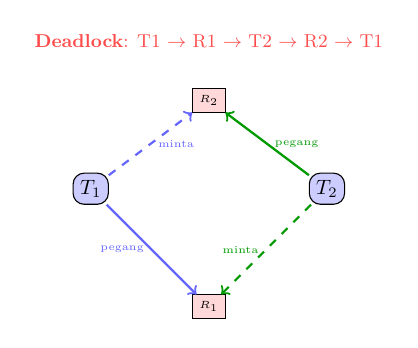
\begin{tikzpicture}[scale=0.75, transform shape]
        \node[draw, fill=blue!20, rounded corners] (t1) at (0,2.5) {$T_1$};
        \node[draw, fill=blue!20, rounded corners] (t2) at (4,2.5) {$T_2$};
        \node[draw, fill=red!15, font=\tiny] (r1) at (2,0.5) {$R_1$};
        \node[draw, fill=red!15, font=\tiny] (r2) at (2,4) {$R_2$};

        \draw[->, thick, blue!60] (t1) -- node[left, font=\tiny]{pegang} (r1);
        \draw[->, thick, green!60!black] (t2) -- node[right, font=\tiny]{pegang} (r2);
        \draw[->, dashed, thick, blue!60] (t1) -- node[right, font=\tiny]{minta} (r2);
        \draw[->, dashed, thick, green!60!black] (t2) -- node[left, font=\tiny]{minta} (r1);

        \node[font=\small, red!70] at (2, 5) {\textbf{Deadlock}: T1 $\to$ R1 $\to$ T2 $\to$ R2 $\to$ T1};
    \end{tikzpicture}
\end{frame}

%--- Slide 27: Strategi pencegahan ---
\begin{frame}
    \frametitle{Cara Mencegah Deadlock}
    \framesubtitle{Langgar salah satu dari empat kondisi}
    \small

    \begin{tabular}{p{2.2cm} p{3.5cm} p{2.8cm}}
        \textbf{Kondisi} & \textbf{Cara Melanggar} & \textbf{Implikasi} \\
        \hline
        Mutual Exclusion & Buat resource tidak eksklusif & Tidak selalu bisa \\
        Hold and Wait & Minta semua resource sekaligus & Boros, efisien turun \\
        No Preemption & Ambil paksa resource & Bisa rusak state \\
        Circular Wait & \tem{Urutan lock konsisten} & \textbf{Praktis} \\
    \end{tabular}

    \vspace{1em}
    \begin{alertblock}{Strategi paling praktis}
        \centering
        \textbf{Urutan lock yang konsisten}.\\
        Jika semua thread mengambil lock A dulu baru B,\\
        maka \tem{circular wait tidak akan pernah terbentuk}.
    \end{alertblock}
\end{frame}

%--- Slide 28: Checkpoint deadlock ---
\begin{frame}[shrink=10]
    \frametitle{Checkpoint: Deadlock}
    \framesubtitle{Tiga pertanyaan — jawab tanpa melihat slide sebelumnya}
    \small

    \begin{enumerate}
        \item Jelaskan empat kondisi yang harus terpenuhi agar deadlock terjadi.
        \item Kapan kita bisa yakin deadlock terjadi hanya dengan melihat Resource Allocation Graph?
        \item Apa strategi paling praktis untuk mencegah deadlock? Jelaskan alasannya.
    \end{enumerate}

    \begin{block}{Jawaban}
        \footnotesize
        \begin{enumerate}
            \item Mutual exclusion, hold and wait, no preemption, circular wait. Keempatnya harus ada bersamaan.
            \item Jika ada cycle dan setiap resource dalam cycle hanya punya satu instance.
            \item Urutan lock konsisten — melanggar circular wait tanpa biaya tinggi.
        \end{enumerate}
    \end{block}
\end{frame}

%================================================
% CLOSING
%================================================
\section{Rangkuman}

\begin{frame}[plain]
    \begin{center}
        \vspace{3cm}
        \Huge\textbf{Rangkuman Week 11}\\[0.4em]
        \Large\textit{Apa yang Sudah Kita Pelajari}
    \end{center}
\end{frame}

\begin{frame}
    \frametitle{Rangkuman}
    \framesubtitle{Lock, Atomic Instructions, dan Deadlock}
    \small

    \begin{block}{Lock}
        \begin{itemize}
            \item Lock punya dua operasi: acquire (lock) dan release (unlock)
            \item \texttt{pthread\_mutex}: sleep-based lock, hemat CPU
            \item Spinlock: busy-wait lock, lebih cepat untuk tunggu singkat
        \end{itemize}
    \end{block}

    \begin{block}{Hardware Foundation}
        \begin{itemize}
            \item Software-only lock gagal karena CHECK dan SET terpisah
            \item Instruksi atomik: Test-and-Set, Compare-and-Swap
            \item Atomic = satu instruksi yang tidak bisa disela
        \end{itemize}
    \end{block}

    \begin{block}{Deadlock}
        \begin{itemize}
            \item Empat kondisi: mutual exclusion, hold \& wait, no preemption, circular wait
            \item Resource Allocation Graph untuk deteksi deadlock
            \item Pencegahan praktis: urutan lock yang konsisten
        \end{itemize}
    \end{block}
\end{frame}

\end{document}
